\documentclass[a4paper]{article}
\usepackage{graphicx}
\usepackage{booktabs}
\usepackage{amsmath}
\usepackage{setspace}
\usepackage{float} 
\usepackage{array}
\usepackage{enumerate}
\usepackage{indentfirst} 
\usepackage[style=mla]{biblatex}
\usepackage{hyperref}
\usepackage{multicol}
\usepackage{multirow}
\usepackage{siunitx}
\usepackage{listings} 
\usepackage{xcolor}
\usepackage{amsmath, amssymb, graphics, setspace}
\usepackage[top=1.2in, bottom=1.2in]{geometry}
\setlength{\parindent}{2em}

\newcommand{\mathsym}[1]{{}}
\newcommand{\unicode}[1]{{}}


\lstset{extendedchars=false}%解决代码跨页时,章节标题,页眉等汉字不显示的问题

\begin{document}

 \begin{titlepage}
  \begin{center}
   \begin{spacing}{2.5}
   \textbf{\huge Lab4 Report}\\[0.5cm]
   \textbf{\Large Pipelined Processor}\\
   \vspace*{\fill}
   \textnormal{Thursday Group 8\\Chunyu Wang\\Weiqing Xu\\Wenbo Yu}
   \end{spacing}

   \begin{spacing}{1.5}
   \textbf{\large \\}
   \textbf{\large \\}
   \vspace*{\fill}
   \renewcommand{\baselinestretch}{1.5}
   \textnormal{\large UM-SJTU Joint Institute \\ ECE3700J Intro to Computer Organization\\}
   \end{spacing}
   
   \begin{spacing}{2.0}
   \textnormal{\large Fall 2022}
   \end{spacing}
  \end{center}
 \end{titlepage}

 \section{Brief Description of Our Modeling and Implementation}
 \paragraph{}Our basic idea is to modify the pipelined processor we have learned in class, as shown in the figure below:
 \begin{figure}[h]
     \centering
     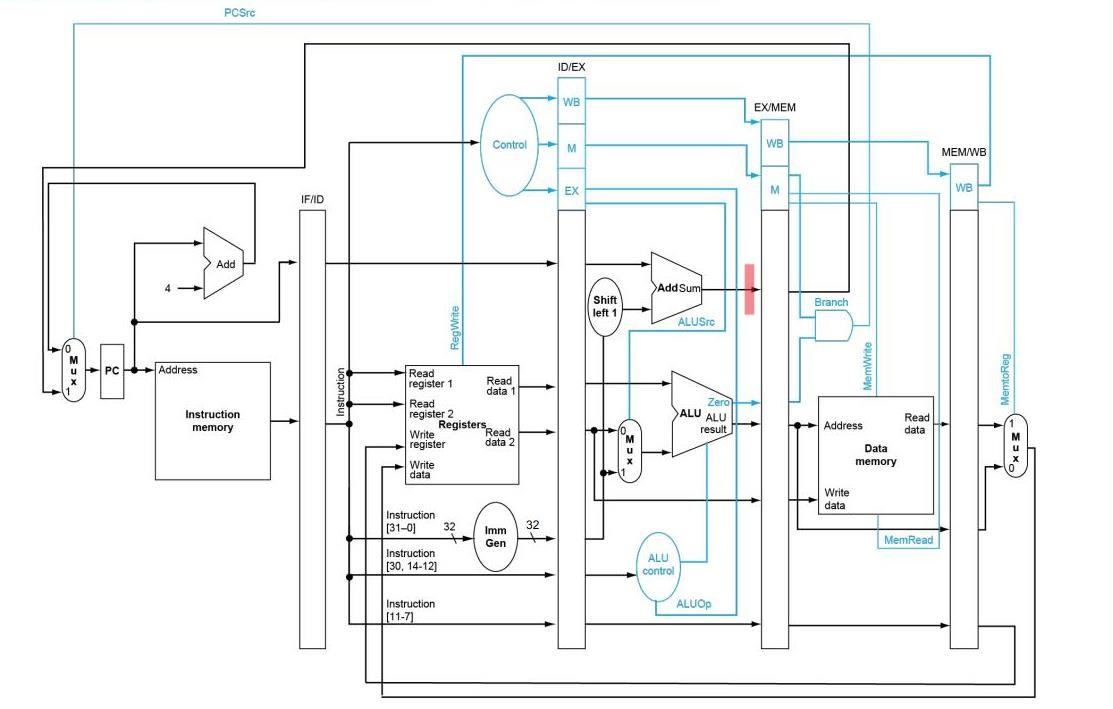
\includegraphics[scale=0.6]{lab4_pp.jpg}
     \caption{Caption}
     \label{fig:1}
 \end{figure}
\paragraph{}To support all the instructions listed in lab manual, we add:
\begin{enumerate}
    \item a new control signal isJump generated by central control, 1 when jalr, otherwise 0.
    \item a 2-to-1 mux in EX stage. The position of the mux is shown in the figure (red thick line). The mux takes the adder result (PC+Imm*2) and ALU result as input data, the jump signal from ID/EX register as selecting signal. The function of this mux is for jalr, since jalr need jump of PC but, as an I-type instruction, the destination can only be calculated by ALU.
    \item 3 bit wire of funct3 to Data Memory, in order to know whether the load or save data is word or byte, or unsigned.
    \item a new input of mux in WB stage, in order to save the next PC when jal and jalr. 
\end{enumerate}

\paragraph{}For other detailed modification, we just need to set the control signal:\\
\begin{tabular}{|c|c|c|c|c|c|c|c|c|}
/ & Branch & ALUSrc & 
ALUOp & MemWrite & MemRead & MemtoReg & Jump & RegWrite \\
I-type:load & 0 & 1 & 00 & 0 & 1 & 01 & 0 & 1 \\
I-type:Imm & 0 & 1 & 11 & 0 & 0 & 00 & 0 & 1 \\
S-type & 0 & 1 & 00 & 1 & 0 & 00 & 0 & 0 \\
B-type & 1 & 0 & 01 & 0 & 0 & 00 & 0 & 0 \\
jalr & 1 & 1 & 00 & 0 & 0 & 10 & 1 & 1 \\
J-type:load & 1 & 1 & 00 & 0 & 0 & 10 & 0 & 1 \\
R-type:load & 0 & 0 & 10 & 0 & 0 & 00 & 0 & 1 \\
\end{tabular}

\begin{tabular}{|c|c|c|c|}
 ALUsel & ALU operation & instruction & Zero\\
 0010 & x1+x2 & add,jal,jalr... & 1 \\
 1000 & x1-x2 & sub,beq & (x1==x2) \\
 1001 & x1-x2 & bne & !(x1==x2) \\
 1100 & x1-x2 & blt & (x1<x2) \\
 1110 & x1-x2 & bge & !(x1<x2) \\
 0100 & x1\^{}x2 & xor & /  \\ 
 0110 & x1\textbar x2 & or & / \\ 
 0111 & x1\&x2 & and & / \\
 0001 & x1\textless \textless x2 & sll & / \\
 0101 & x1\textgreater \textgreater x2 & srl & / \\
 1101 & x1\textgreater \textgreater x2 (sign extension) & sra & /
\end{tabular}

 \end{document}